\section{Implementation}
\label{sec:Implementation}

For evaluating the proposed system, we created \textit{Pallidor} a prototypical implementation using the Swift programming language. It is composed of multiple subsystems that are developed and maintained as standalone Swift packages. Each package provides the functionality of a subsystem that is defined in Section \ref{ch:SystemDesign}. \texttt{PallidorGenerator} implements the \texttt{IDL Conversion} and \texttt{IDL Importer} subsystems. Migrating a previously generated facade is performed by the \texttt{Pal\-lidor\-Migrator} package that provides the services of the \texttt{Migration Ma\-na\-ger}, \texttt{Migration Guide Importer} and \texttt{SourceCode Importer} subsystems. 

\begin{figure}[!h]
	\centering{
		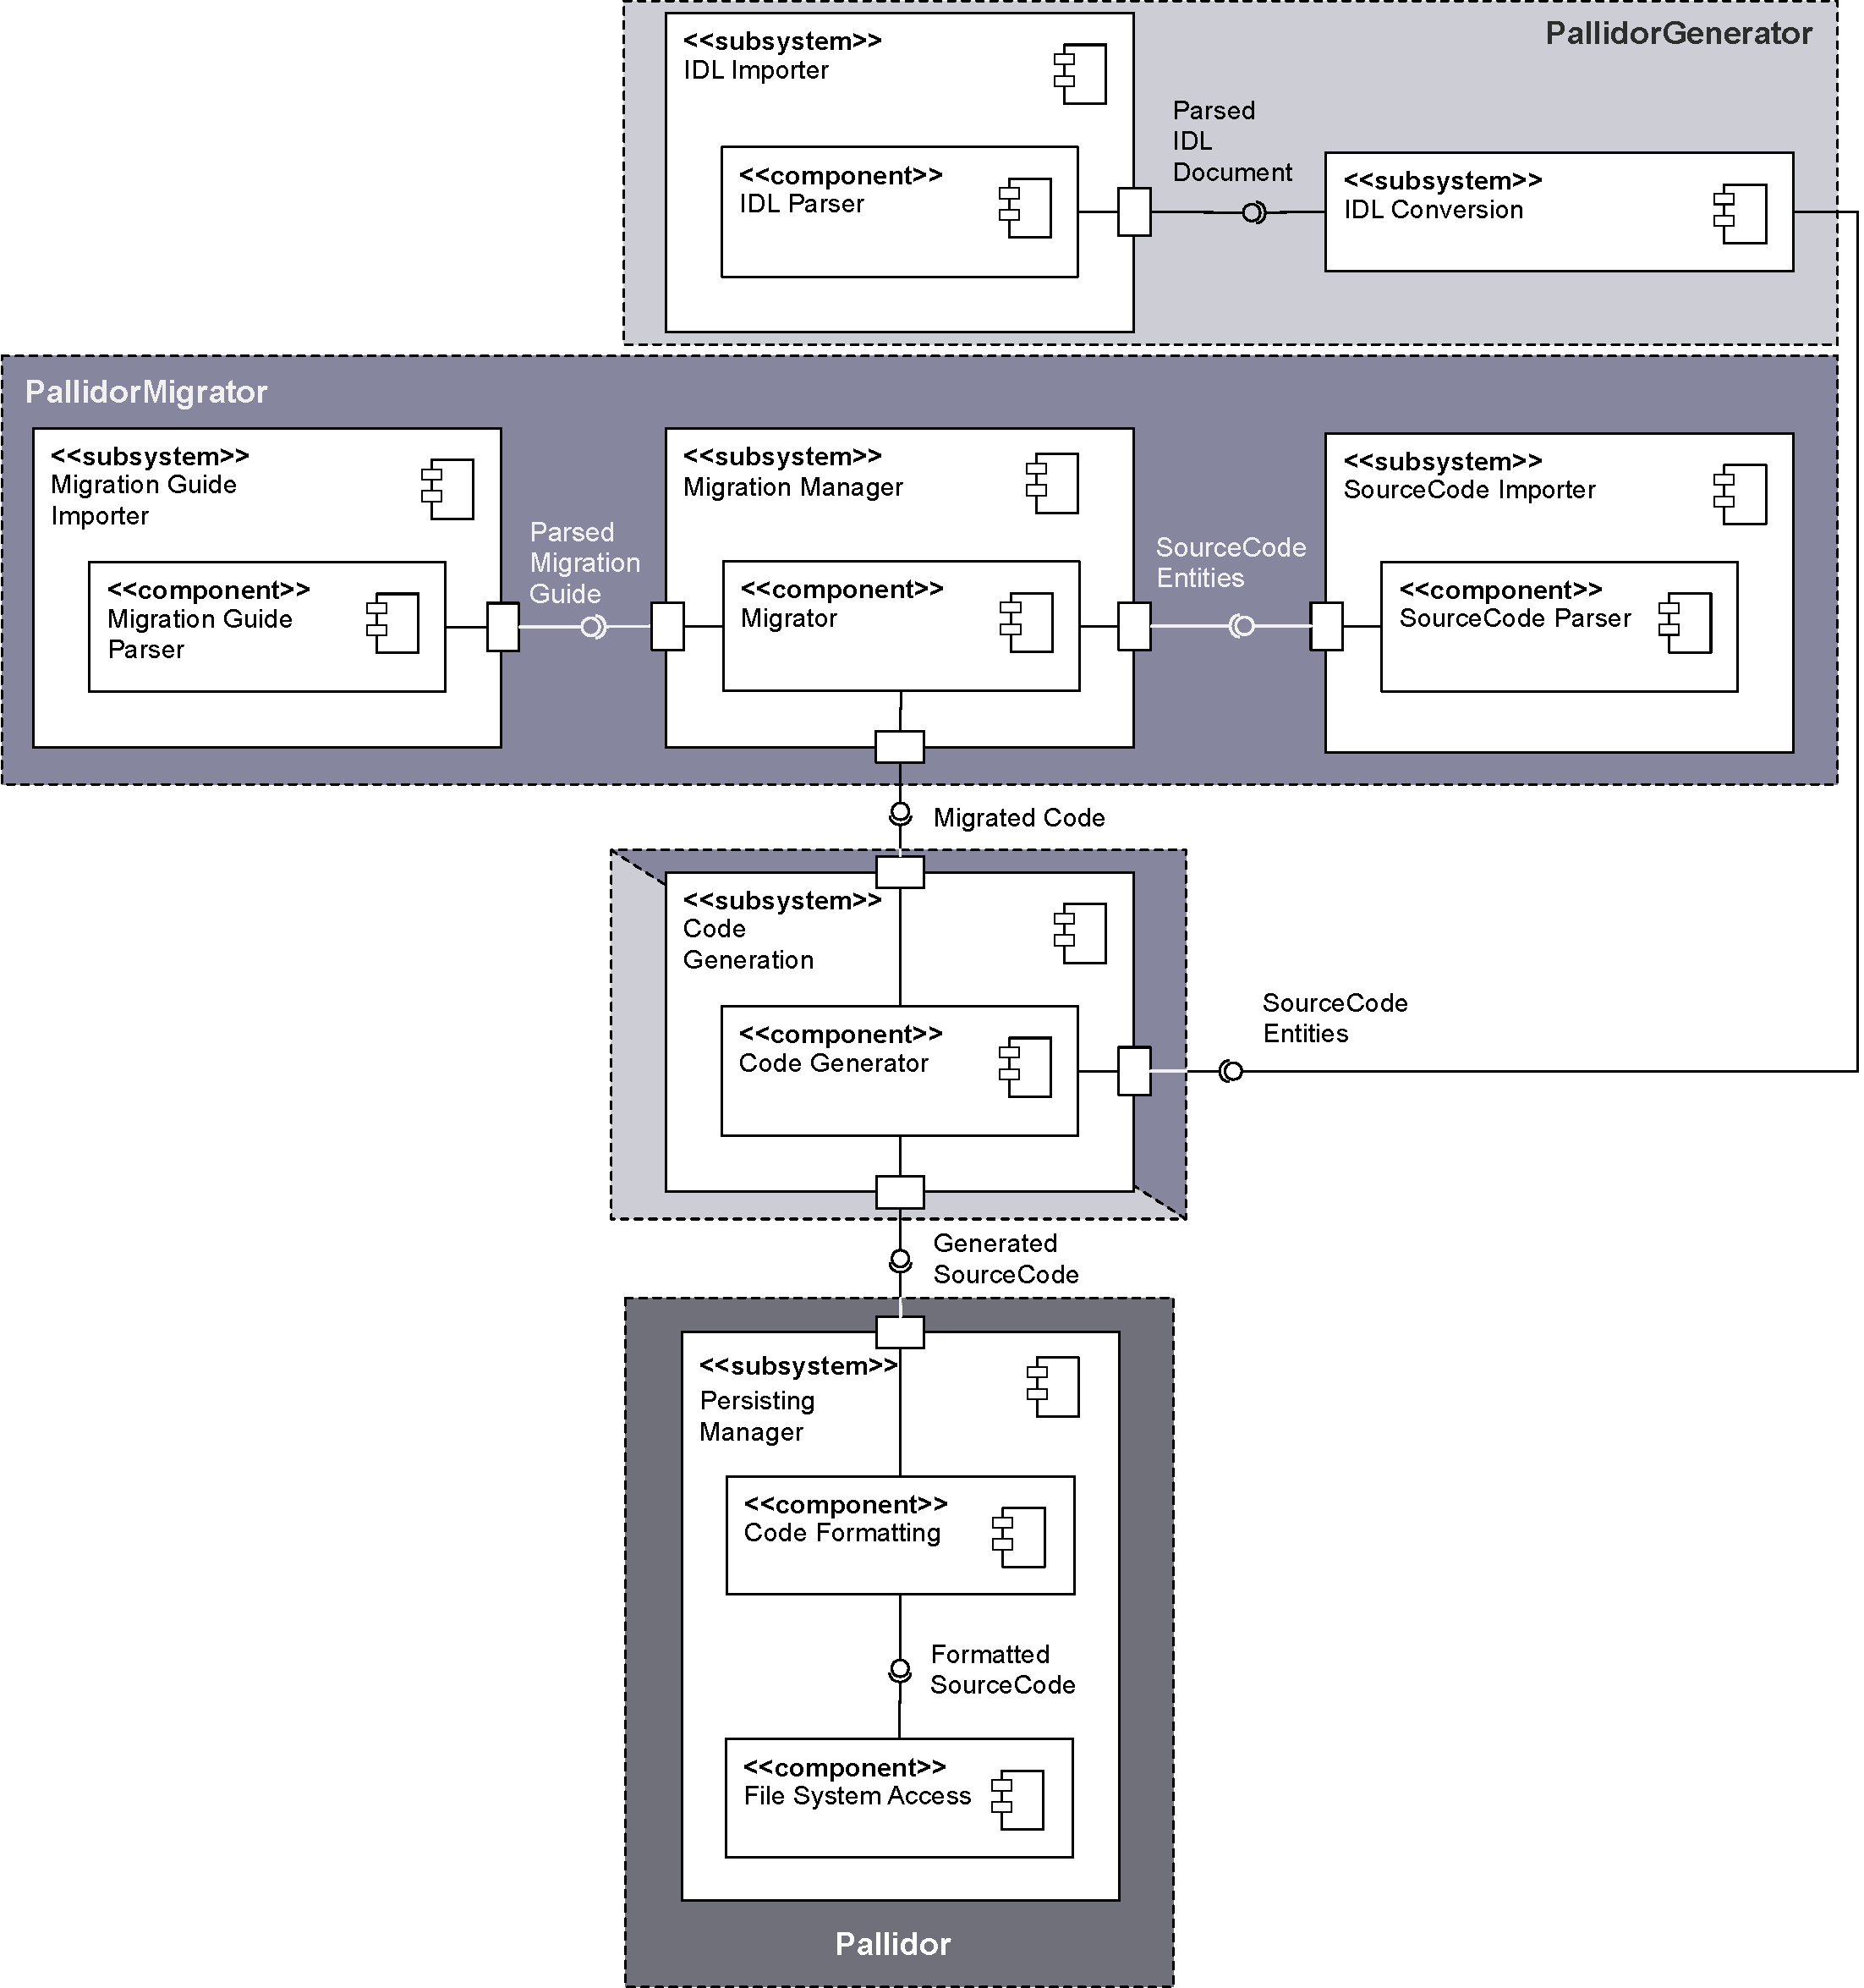
\includegraphics[width=140mm]{images/subsystem_implementation.pdf}
		\caption{Implementation of subsystems with Pallidor Swift packages}
		\label{fig:subsystemImplementation}
	}
\end{figure}
Both packages implement the functionality of the \texttt{Code Generation} subsystem and persist their respective results in files. The \texttt{Code Generation} subsystem is not separately implemented because our prototype only supports the Swift programming language. The \texttt{Pallidor} package combines both subpackages in an executable that provides a commandline user interface. Furthermore, it formats the source code and persists it afterwards. Figure \ref{fig:subsystemImplementation} illustrates which package implements the respective subsystem.  

In addition to our own implementations, third-party open source components that provide the required functionality are integrated using the Swift Package Manager. Key components and their respective implemented subsystems are listed in Table \ref{tbl:PallidorDep}. Since Pallidor is a prototype, its functionality is limited to generating a persistent Swift package from an OpenAPI specification. It can be integrated in client applications using Swift in version 5.2 or later. Since our generated Swift package uses Apple's \texttt{Combine}\footnote{https://developer.apple.com/documentation/combine} framework, the client application's execution environment must be at least iOS 13 or MacOS 10.15. 

\renewcommand{\arraystretch}{1.4}
\begin{table*}[ht]
	\begin{center}
		\begin{tabular}{|>{\centering\arraybackslash}m{2.7cm}|>{\centering\arraybackslash}m{3cm}|>{\centering\arraybackslash}m{3.2cm}|>{\centering\arraybackslash}m{4cm}|}
			\hline
			\begin{center}
				\textbf{Subsystem/ Component}
			\end{center} &  \begin{center}
				\textbf{Swift Package Name} 
			\end{center}&  \begin{center}
				\textbf{Swift Package Version}
			\end{center} &
		 \begin{center}
			\textbf{Swift Package Author / Publisher}
		\end{center} \\ \hline
			\textit{IDL Importer} & OpenAPIKit & 2.2.0 \newline (Dec. 20th, 2020) &
			Mathew Polzin \\ \hline
			\textit{Source Code Importer} & Sourcery & 1.0.2 \newline (Nov. 30th, 2020) &
			Krzysztof Zabłocki \\ \hline
			\textit{Code Formatter} & swift-format & 0.50300.0 \newline (Sep. 19th, 2020) &
			Apple, Inc. \\ \hline
		\end{tabular}
		\caption{Third-party Swift packages used for subsystems in Pallidor}\label{tbl:PallidorDep}
	\end{center}
\end{table*}

The \texttt{OpenAPIKit} is a library that enables encoding to- and decoding Swift types from OpenAPI documents. It supports importing documents structured in JSON and YAML formats and provides Swift types for most types of the OpenAPI specification in (3.0.2). In its latest version, the \texttt{OpenAPIKit} does not support \texttt{Link Objects} and specification extensions for \texttt{OpenAPI.XML} and \texttt{OpenAPI.Oauth\-Flows}. As opposed to the OpenAPI specification, this library specifies the \texttt{re\-qui\-red} property of schema elements on the element instead of the parent object. OpenAPI documents must be provided as \texttt{Data} or \texttt{String} types, as the \texttt{OpenAPIKit} does not support reading files. Furthermore, all reference elements (\texttt{\$ref}) must be internal references and target the same file in order to be resolved.

\texttt{Sourcery} is a code generator for Swift, built on top of Apple's \texttt{SourceKit}. It extends its functionality and types to facilitate generating Swift code based on Stencil templates. Although \texttt{Sourcery} is designed as a commandline tool to be integrated in a custom build phase, it provides a framework that can be incorporated using the Swift Package Manager. In addition to generating Swift code, it provides support for parsing Swift strings in corresponding source code entities. 

Formatting the generated Swift code is performed by \texttt{swift-format}. It can be used as a commandline tool or integrated into applications using the Swift Package Manager. It provides an API to format Swift code according to a style configuration. If no set of styling rules is specified, a default style is used. The package is compatible with Swift 5.1 and higher and requires selecting the appropriate branch that corresponds to the version of Swift used in the integrating application.

\subsection{Pallidor Generator}\label{subsec:PallidorGenerator}

The \texttt{PallidorGenerator} Swift package is concerned with retrieving and parsing of OpenAPI specifications to generate the library layer of the Swift package for the client application. Therefore, OpenAPI specifications must be parsed and converted to source code entities. After that, they are transformed into source code strings in the Swift programming language and are persisted in files. The package integrates the \texttt{OpenAPIKit} which decodes an OpenAPI specification in its \texttt{Open\-API.Document} type. This type is composed of elements that represent the attributes of an OpenAPI specification. Furthermore, it provides a locally dereferenced representation that facilitates the traversal of its structure by replacing all \texttt{\$ref} elements with their referenced entities. The \texttt{OpenAPI.Document} needs to be converted to source code entities before Swift code can be generated. This conversion is performed during the traversal of the document by using various \texttt{Resolver} objects. Depending on the OpenAPI specification element that needs to be converted, a corresponding \texttt{Resolver} initializes a source code entity model using the information of the OpenAPI element. Resolving an endpoint struct from the \texttt{Resolved\-Route} type of the \texttt{OpenAPIKit} is shown in Listing \ref{lst:Resolving}.

\begin{lstlisting}[language=Swift, caption={Resolving an operation}, captionpos=b, label={lst:Resolving}]
	/// Resolves an endpoint struct
	/// - Parameters:
	///   - path: path in OpenAPI document
	///   - route: Resolved route from OpenAPI document
	/// - Returns: resolved EndpointModel
	static func resolve(path: OpenAPI.Path, route: ResolvedRoute) -> EndpointModel {
		let endpoint = EndpointModel(
				name: path.components[0].upperFirst(), 
				operations: [], 
				detail: route.summary)
		endpoint.operations = route.endpoints.map( 
				{ OperationModel.resolve(endpoint: $0) })
		return endpoint
	}

\end{lstlisting}

All source code entity models of the \texttt{PallidorGenerator} package are extended with the \texttt{Custom\-String\-Convertible} protocol that adds the \texttt{description} computed property. It is used to specify string templates for generating the Swift code of the library layer. They are dynamically composed of all string templates of nested models such as methods, parameters or properties. Furthermore, static templates for meta files such as the \texttt{Package.swift} file are provided as Markdown (\texttt{.md}) files. Although minor adjustments are made, for example specifying the name of the Swift package, their functionality remains the same between different Web APIs.

\begin{lstlisting}[language=Swift, caption={Source code string template for an endpoint}, captionpos=b, label={lst:EndpointTempl}]
	/// Extension of the Endpoint Model
	/// Used for generating client library code in Swift
	extension EndpointModel : CustomStringConvertible {
		var description: String {
			"""
			import Foundation
			import Combine
			
			struct _\(name.upperFirst())API {
				static let decoder ...
				\(operations
				.sorted(by: {$0.operationId < $1.operationId})
				.map({$0.description})
				.joined())
			}
			"""
		}
	}

\end{lstlisting}

The public interface of the \texttt{PallidorGenerator} Swift package is provided by the file of the same name. Its initialization requires specifying the URL of the OpenAPI specification to be decoded. Depending on its format, a \texttt{JSON\-Decoder} or \texttt{YAML\-Decoder} is created that is used to decode the OpenAPI specification. Initializating the \texttt{Pal\-li\-dor\-Gen\-er\-ator} fails, if the OpenAPI document cannot be decoded or resolved due to an invalid URL or malformed structure. Generating the Swift code of the library layer and persisting it in files is performed by invoking its \texttt{generate} method. It receives a \texttt{path} parameter and the name of the client library as specified by the user. After generating all files, a list of their URLs is returned to the method's caller. The method throws an error if writing the files in the target directory fails. Several OpenAPI specifications of various Web APIs are used for testing the \texttt{PallidorGenerator} Swift package. They are specified in Markdown files and are located in the \texttt{Resources} subfolder of the test folder. The generated files are validated against predefined results specified in Markdown files that are located in the \texttt{Results} subfolder. 

Integrating the \texttt{PallidorGenerator} package in a Swift project, the URL of its GitHub repository must be added to the dependencies in the \texttt{Package.swift} file. Furthermore, the \texttt{develop} branch must be selected for using its latest version.
\newpage
\begin{lstlisting}[language=Swift, caption={Integrating PallidorGenerator in SPM}, captionpos=b, label={lst:IntegrationGenerator}]
	.package(
			url: "https://github.com/Apodini/PallidorGenerator.git", 
			.branch("develop")
	)
\end{lstlisting}


With regard to the implementation of the \texttt{PallidorGenerator} Swift package, some restrictions must be observed. Instead of defining inline objects in nested elements of an OpenAPI specification, schema components must be used to specify custom data types. They must be referenced at their designated target element. This limitation is based on the problem that nested elements do not provide an identification, which is required for building the library layer. The Open\-API specification supports defining primitive data types as schema components using a custom name. These type aliases are resolved and their underlying primitive types are used in the generated client library. Furthermore, all endpoint methods in an Open\-API specification must specify the \texttt{operationId} property. Analogous to schema components, this identifier is used by \textsc{Pallidor} to recognize changes and to generate the client library. Although it is not enforced by the OpenAPI specification, all operations must specify at least one response that is returned after the request was processed successfully. Otherwise the return value type of an operation cannot be inferred from the Open\-API document. Unlike successful responses, error responses can be of various types.
\subsection{Pallidor Migrator}\label{subsec:PallidorMigrator}

The \texttt{PallidorMigrator} package integrates the functionality of the \texttt{Migration} \texttt{Ma\-nager}, \texttt{Migration Guide Importer} and \texttt{SourceCode Importer} subsystems. It uses the information stated in the parsed migration guide to adapt the source code entities of a previously generated facade layer. Therefore, a set of migrations is initialized that performs the necessary migratory steps on the changed target properties of the source code entity. After migrating all changes, the source code entities are converted into Swift code that gets persisted in files. The machine-readable migration guide is parsed by the builtin \texttt{JSONDecoder} of Swift's \texttt{Foundation} framework. The \texttt{PallidorMigrator} package provides a model for mapping the migration guide to its decoded representation. Depending on the type of change that is stated in the migration guide, the \texttt{MigrationSet} initializes a corresponding \texttt{Migration} object. Each \texttt{Migration} is checked for plausiblity on its initialization. Thereby, invalid or inconsistent changes are detected and its \texttt{solvable} property is set to false. An unsolvable \texttt{Migration} results in an error message that is propagated to the user. Every \texttt{Migration} targets one source code entity of a previously generated facade. The \texttt{Sourcery} framework is used for importing its source code. It provides source code entities for all syntactical elements of Swift code such as classes, structs and methods. These entities cannot be extended within the \texttt{PallidorMigrator} package, because they are declared as \texttt{final}.

\begin{lstlisting}[language=Swift, caption={Extending a wrapped Sourcery struct}, captionpos=b, label={lst:WrappedStruct}]
	/// Wraps struct types of Sourcery
	class WrappedStruct: Modifiable {
		...
		convenience init(from: SourceryRuntime.Struct) {
			self.init(
				localName: from.localName.removePrefix, 
				variables: from.variables
					.map({ WrappedVariable(from: $0) }), 
				methods: from.methods
					.map({ WrappedMethod(from: $0) }))
		}
	}
\end{lstlisting}

In order to adapt them to changes, wrapper classes are used to extend their functionality with the \texttt{Modifiable} protocol. This protocol introduces a \texttt{modify} method that receives a \texttt{Change} object as a parameter. A modifiable endpoint struct that wraps the \texttt{SourceryRuntime.\-Struct} type of the \texttt{Sourcery} framework is shown in Listing \ref{lst:WrappedStruct}. Depending on the type of change that the \texttt{modify} method receives, the corresponding handling routine is performed. 

\begin{lstlisting}[language=Swift, caption={Modification of a changed method entity}, captionpos=b, label={lst:MethodModify}]
	/// Wrapped method of SourceryMethod
	class WrappedMethod: Modifiable {
		...
		func modify(change: Change) {
			self.modified = true
			switch change.changeType {
				case .add:
					handleAddChange(change: change as! AddChange)
					break
				case .rename:
					handleRenameChange(change: change as! RenameChange)
					break
				case .replace:
					handleReplaceChange(change: change as! ReplaceChange)
					break
				case .delete:
					handleDeleteChange(change: change as! DeleteChange)
					break
			}
		}
	}
\end{lstlisting}

Their implementations vary depending on the type of source code entity that is modified. They adapt an entity's associated properties according to the details of the migration. In Listing \ref{lst:MethodModify}, the implementation of the \texttt{modify} method highlights the various handling routines that are used to migrate the properties of a \texttt{WrappedMethod}. Similar to the source code entities of the \texttt{PallidorGenerator} package, the wrapped source code entities provide templates that are used to convert them into Swift code. These source code strings are persisted in files.

The public interface of the \texttt{PallidorMigrator} Swift package is provided by the file of the same name. Its initialization requires specifying the URL of the migration guide and the URL of the directory in which the previously generated client library is located. If the migration guide cannot be retrieved or decoded, an error message is thrown and forwarded to the user. Furthermore, on initialization of the \texttt{PallidorMigrator} struct a set of migrations is created. If their plausibility check fails, an error message is shown to the user. Migrating the changes as stated in the migration guide and persisting the adapted facade layer in files are started by invoking the \texttt{buildFacade} method. After generating all files, it returns a list of their URLs. An error is thrown if writing the files of the adapted facade layer fails. The \texttt{PallidorMigrator} Swift package is extensively tested to discover erroneousness migrations. Therefore, migration guides are created that contain various types of changes with their respective targets. The unit tests migrate prepared source code entities according to these migration guides and compare the outcome to predefined results. Various integration tests are performed that combine different changes on a single target to ensure that they do not affect each other. The input documents of previously generated facade layer code and their predefined adapted results are specified in Markdown files located in the \texttt{Resources} subfolder of the test folder. 

Integrating the \texttt{PallidorMigrator} package in a Swift project, the URL of its GitHub repository must be added to the dependencies in the \texttt{Package.swift} file. Furthermore, the \texttt{develop} branch must be selected for using its latest version.

\begin{lstlisting}[language=Swift, caption={Integrating PallidorMigrator in SPM}, captionpos=b, label={lst:IntegrationMigrator}]
	.package(
		url: "https://github.com/Apodini/PallidorMigrator.git", 
		.branch("develop")
	)
\end{lstlisting}

The implementation of the \texttt{PallidorMigrator} Swift package deviates from the design of our proposed system. In addition to the original design, the generated library layer must also be imported. No migration guide or previously generated facade can be used during the initial integration of \textsc{Pallidor} as the current version of the Web API is persisted. Therefore, the facade layer is generated based on the public interface of the library layer. Furthermore, no migration strategy can be selected so that all changes of a WebAPI are migrated. A limitation of \texttt{Sourcery} concerns the automatic documentation of the public facade layer of the client library because it does not support parsing comment annotations. Therefore, the documentation for the client library is located at the library layer and must be consulted manually. Additionally, some types of migration must be performed by combining multiple migratory steps. Replacing an endpoint is achieved by replacing all of its methods and then renaming it. Renaming and replacing enum cases and inherited schemas is accomplished by adding their replacements before removing them. Return values of endpoint methods can only be replaced because they do not specify a name that could be renamed. Furthermore, all operations must provide a return value type, which means that deleting them or adding them later is not applicable.
\subsection{Pallidor}\label{subsec:Pallidor}
The \textsc{Pallidor} package contains the command-line user interface and the \texttt{Code\- Formatting} component. Furthermore, it stores all configuration settings of the user. By invoking \textsc{Pallidor} via its commandline interface and providing all required configuration parameters, the client library is generated. The \texttt{swift\-argument-parser}\footnote{https://github.com/apple/swift-argument-parser} package is used to supply detailed error and help messages and it facilitates type-safe argument parsing. The URLs of the OpenAPI specification and migration guide are used to initialize the \texttt{Pallidor\-Generator} and \texttt{Pallidor\-Migrator} Swift packages. Additionally, the name and location of the client library are used by the packages to both, import previously generated source code and persist their results after execution. After both packages successfully completed their tasks, the \texttt{swift-format} package is used to format the code according to the ruleset that the user provided. The formatted source code strings overwrite the previously generated Swift files.

Several parameters are used to configure \textsc{Pallidor}. While the URLs of the migration guide, OpenAPI specification and location of the package as well as its name are mandatory parameters, specifying a ruleset for formatting the source code strings is optional. \textsc{Pallidor} is limited to emitting the client library as a Swift package, hence selecting a programming language currently defaults to Swift. A migration strategy can be set to exclude certain types of migration. This configuration parameter defaults to the implemented strategy of migrating all types. The \texttt{help} argument is provided by the \texttt{swift-argument-parser} and lists all available parameters of \textsc{Pallidor}. It also supports the user with helpful error messages that highlight the correct usage.

\begin{lstlisting}[language=Tex, caption={Command-line arguments of Pallidor to support user}, captionpos=b, label={lst:arguments}]
	Error: Missing expected argument 
				'--target-directory <target-directory>'
	
	USAGE: pallidor 
	--openapi-specification-url <openapi-specification-url> 
	--migration-guide-url <migration-guide-url>
	--target-directory <target-directory> 
	--package-name <package-name> 
	[--language <language>] 
	[--strategy <strategy>]
	[--custom-formatting-rule-path <custom-formatting-rule-path>]
	
	OPTIONS:
	-c, --custom-formatting-rule-path <custom-formatting-rule-path>
	If you want to use your own code formatting rules, specify path here 
	-o, --openapi-specification-url <openapi-specification-url>
	URL of OpenAPI specification of the package to be generated 
	-m, --migration-guide-url <migration-guide-url>
	URL of migration guide of the package to be generated 
	-t, --target-directory <target-directory>
	Output path of the package generated 
	-p, --package-name <package-name>
	Name of the package generated 
	-l, --language <language>
	Programming language that the client library should be generated in (default: Swift)
	-s, --strategy <strategy>
	Migration strategy that excludes certain types of change from being migrated (default: all)
	-h, --help
	Show help information.

\end{lstlisting}

\textsc{Pallidor} is designed as a command-line tool that can be integrated into an existing CI/CD system. Therefore, it needs to be compiled and the binaries must be deployed. The configuration parameters can be predefined in a script file that is integrated in the build phase of the CI pipeline. The script is automatically executed as a step phase and performs the migration to generate the Swift package that is integrated in the client application. The CI/CD system must be configured to publish the generated Swift package in a separate respository that is referenced from the \texttt{Package.swift} file of the client application. After that it automatically creates a new release of the client application.


